\باب{سمتیات عارضی باب}
%+++++++++++++++++++++++++++++++++++++++++++++++++++++++++++++++++
%++++++++++++++++++++++++++++++++++++++++++++++++++++++++++++++++
this is sec 9.1 to 9.4 of the latest addition. i shall palce it at the very beginning of my 7th chapter.this resolves all the issues.
%++++++++++++++++++++++++++++++++++++++++++++++++++++++++
%++++++++++++++++++++++++++++++++++++++++++++++++++++++++++
%++++++++++++++++++++++++++++++++++++++++++++++++++++++
%++++++++++++++++++++++++++++++++++++++++++++++++++++++++++++++++
\حصہ{غیر سمتیات اور سمتیات}
طبیعیات اور جیومیٹری میں ایسی قیمتیں پائی جاتی ہیں جنہیں ان کی مقدار سے مکمل طور پر بیان کیا جا سکتا ہے۔مثلاً  کمیت، درجہ حرارت، برقی بار، وقت، رقبہ، حجم، فاصلہ، برقی دباو وغیرہ۔ان میں سے ہر ایک کو (مقدار کی موزوں اکائی چن کر) ایک عدد  سے ظاہر کیا جا سکتا ہے۔ ایسی تمام مقداروں کو \اصطلاح{غیر سمتیات}\فرہنگ{غیر سمتیات}\فرہنگ{سمتیہ!غیر}\حاشیہب{scalars}\فرہنگ{scalars} کہتے ہیں۔غیر سمتی مقدار کی قیمت پر چننی گئی محدد کا کوئی اثر نہیں ہو گا۔

اس کے برعکس طبیعیات اور جیومیٹری میں ایسی قیمتیں بھی پائی جاتی ہیں جن کی مکمل اظہار کے لئے ان کی قیمت کے علاوہ ان کی سمت بھی درکار ہوتی ہے۔ان کی ایک مثال میکانی  قوت ہے۔ آپ جانتے ہیں کہ قوت کو تیر کی نشان سے ظاہر کیا جا سکتا ہے جہاں تیر کی سمت، قوت کی سمت اور تیر کی لمبائی (کسی پیمائش کے تحت) قوت کی مقدار کو ظاہر کرتی ہے۔ شکل \حوالہ{شکل_الجبرا_قوت_سمتی_رفتار}-الف میں ہلکے دھاگے سے بندھی ہوئی کمیت \عددی{m} کی دائری حرکت دکھائی گئی ہے۔کمیت کی لمحاتی سمتی رفتار \عددی{\bM{v}} کو تیر سے دکھایا گیا ہے۔اس تیر کی سمت، کمیت کی لمحاتی سمتی رفتار دیتی ہے جبکہ تیر کی لمبائی (کسی موزوں تناسب سے) لمحاتی سمتی رفتار کی قیمت دیتی ہے۔شکل میں کمیت کی اسراع \عددی{\bM{a}} بھی دکھائی گئی ہے جہاں \عددی{\bM{a}} کی لمبائی (کسی موزوں تناسب سے) لمحاتی اسراع کی قیمت دیتی ہے۔

سیدھی سطح میں تکون کی (بلا گھومے) منتقلی شکل \حوالہ{شکل_الجبرا_قوت_سمتی_رفتار}-ب میں  دکھائی گئی ہے۔اس حرکت کو (تکون کے ہر نقطے کی) طے فاصلے  کی مقدار اور سمت سے ظاہر کیا جا سکتا ہے۔تکون پر کسی نقطے کی ابتدائی مقام \عددی{A} سے اختتامی مقام \عددی{B} تک سمتی خط سے اس حرکت کو ظاہر کیا جا سکتا ہے۔یوں سمتی خط \عددی{\bM{b}}، تکون کے ایک نقطہ کی \عددی{A} سے \عددی{B} منتقلی دکھاتی ہے۔تکون کے ہر نقطے کی ابتدائی مقام سے اختتامی مقام تک سمتی خطوط کھینچ کر ہمیں سمتی خطوط کی نسل ملتی ہے جس میں تمام سمتی  خطوط کی لمبائی ایک جیسی  اور  سمت  ایک جیسی ہو گی (یعنی یہ آپس میں متوازی ہوں گے)۔ ہم کہہ سکتے ہیں کہ ان میں سے ہر ایک سمتی خط، تکون کے ایک نقطے کی ابتدائی مقام سے اختتامی مقام تک منتقلی کو ظاہر کرتی ہے۔ 


اس سے سمتیہ کی درج ذیل تعریف بیان کی جا سکتی ہے۔
\begin{figure}
\centering
\begin{subfigure}{0.5\textwidth}
\centering
\begin{tikzpicture}
\draw[dashed] (0,0) circle (1cm);
\draw[gray](0,0)--++(30:1cm)node[circ]{}node[right,color=black]{\RL{کمیت $m$}};
\draw[-latex](30:1cm)--++(120:0.75cm)node[above]{$\bM{v}$};
\draw[-latex](30:1cm)--++(30:-0.5cm)node[below]{$\bM{a}$};
\end{tikzpicture}
\caption*{(الف) سمتی رفتار اور اسراع۔}
\end{subfigure}%
\begin{subfigure}{0.5\textwidth}
\centering
\begin{tikzpicture}
\draw(0,0)--++(1.5,0)--++(0,1)--++(-1.5,-1);
\draw(15:3)--++(1.5,0)--++(0,1)--++(-1.5,-1);
\draw[-latex](1.5,0.25)node[ocirc]{}node[below right]{$A$}--++(15:3)node[ocirc]{}node[below right]{$B$}node[pos=0.4,below]{$\bM{b}$};
\end{tikzpicture}
\caption*{(ب) سمتیہ کی دم اور  سر۔}
\end{subfigure}%
\caption{سمتیہ کی تفصیل۔}
\label{شکل_الجبرا_قوت_سمتی_رفتار}
\end{figure}
%=================
\ابتدا{تعریف}\quad سمتیہ\\
سمتی خط کو \اصطلاح{سمتیہ}\فرہنگ{سمتیہ}\حاشیہب{vector}\فرہنگ{vector} کہتے ہیں۔اس کی لمبائی کو سمتیہ کی \اصطلاح{لمبائی} اور سمت کو سمتیہ کی \اصطلاح{سمت} کہتے ہیں۔دو سمتیات صرف اور صرف اس صورت ایک دوسرے کے برابر ہوں گے جب ان کی لمبائی ایک جیسی ہو اور ان کی سمت ایک جیسی ہو۔

سمتیہ کی لمبائی کو سمتیہ کی \اصطلاح{اقلیدسی معیار}\فرہنگ{اقلیدسی معیار}\حاشیہب{Euclidean norm}\فرہنگ{Euclidean norm} (یا معیار) اور سمتیہ کی \اصطلاح{مقدار}\فرہنگ{مقدار!سمتیہ}\فرہنگ{سمتیہ!مقدار}\حاشیہب{magnitude}\فرہنگ{magnitude} بھی کہتے ہیں۔
\انتہا{تعریف}  
%=========================

سمتیہ کی ابتدائی نقطے کو سمتیہ کی \اصطلاح{دم}\فرہنگ{دم}\فرہنگ{سمتیہ!دم}\حاشیہب{tail}\فرہنگ{tail} اور اختتامی نقطے کو سمتیہ کا \اصطلاح{سر}\فرہنگ{سر}\فرہنگ{سمتیہ!سر}\حاشیہب{head}\فرہنگ{head} کہتے ہیں۔ یوں شکل \حوالہ{شکل_الجبرا_قوت_سمتی_رفتار}-ب میں نقطہ \عددی{B} سمتیہ \عددی{\bM{b}} کی دم  ہے جبکہ نقطہ \عددی{A} اس کا سر  ہے۔

ہم سمتیات کو موٹی لکھائی میں چھوٹی حروف تہجی مثلاً \عددی{\bM{a}}، \عددی{\bM{b}}، \عددی{\bM{v}}، وغیرہ،  سے ظاہر کرتے ہیں۔ قلم و کاغذ استعمال کرتے ہوئے سمتیہ پر تیر  یا آدھے تیر کا نشان بنایا جاتا ہے یوں اسراع کو \عددیء{\vec{a}} یا  
$\overset{\rightharpoonup}{\rule{0pt}{.9ex}\smash{a}}$
لکھا جاتا ہے۔سمتیہ \عددی{\bM{a}} کی مقدار کو \عددی{\abs{\bM{a}}} لکھا جاتا ہے۔

سمتیہ کی تعریف سے ظاہر ہے کہ ہم سمتیہ کو بغیر گھمائے  ایک جگہ سے دوسری جگہ منتقل کر سکتے ہیں\حاشیہد{یہاں یہ بتلانا ضروری ہے کہ طبیعیات اور جیومیٹری میں ایسی صورتیں پائی جاتی ہیں جہاں سمتیہ  کو ایک جگہ سے دوسری  جگہ منتقل کرنا ممکن نہیں ہوتا ہے۔آپ میکانیات سے جانتے ہیں کہ کسی بھی غیر لچکدار مادے پر قوت کا اطلاق، قوت کی سمت میں لکیر پر رہتے ہوئے،  کسی بھی نقطے پر کیا جا سکتا ہے۔اس سے \اصطلاح{قابل منتقلی سمتیہ}\فرہنگ{سمتیہ!قابل منتقلی}\فرہنگ{vector!sliding} کا تصور پیدا ہوتا ہے۔اس کے برعکس، لچکدار مادے پر قوت کے اطلاق کا نقطہ تبدیل کرنے سے نتائج تبدیل ہوں گے  جو نا قابل قبول بات ہے۔یہ حقیقت \اصطلاح{مقید سمتیہ}\فرہنگ{مقید!سمتیہ}\فرہنگ{سمتیہ!مقید}\فرہنگ{bound vector}\فرہنگ{vector!bound} کی تصور کو جنم دیتی ہے۔اس کتاب میں صرف قابل منتقلی سمتیات پر بات کی جائے گی۔} یعنی ہم سمتیہ کی دم کہیں پر بھی منتقل کر سکتے ہیں۔ظاہر ہے کہ سمتیہ کی دم کا مقام مقرر کرنے سے اس کی سر کا مقام بھی مقرر ہو گا۔

اگر دو سمتیات \عددی{\bM{a}} اور \عددی{\bM{b}} ایک دوسرے کے برابر ہوں تب ہم درج ذیل لکھتے ہیں
\begin{align}
\bM{a}=\bM{b}
\end{align}
اور اگر یہ آپس میں برابر نہ ہوں تب ہم درج ذیل لکھتے ہیں۔
\begin{align}
\bM{a}\ne\bM{b}
\end{align}
کسی بھی سمتیہ کو ترسیمی طور پر موزوں  لمبائی اور سمت کی سمتی خط سے ظاہر کیا جا سکتا ہے۔

ایسا سمتیہ جس کی لمبائی اکائی \عددی{(1)} ہو \اصطلاح{اکائی سمتیہ}\فرہنگ{اکائی!سمتیہ}\فرہنگ{سمتیہ!اکائی}\حاشیہب{unit vector}\فرہنگ{vector!unit}\فرہنگ{unit!vector} کہلاتا ہے۔

%======================
\حصہ{سمتیہ کے اجزاء}
تین بُعدی فضا میں نقطہ ایک جیومیٹریائی چیز ہے جس کو محددی نظام میں تین مرتب اعداد (تصور کیا جا سکتا ہے یا) سے ظاہر  کیا جا سکتا ہے۔ گزشتہ حصے میں ہم نے سمتیہ کی تعریف جیومیٹریائی انداز میں پیش کی، جسے محددی نظام کی استعمال سے الجبرائی انداز میں بھی پیش کیا جا سکتا ہے۔

 نظام محدد  کے \اصطلاح{محور}\فرہنگ{محور}\حاشیہب{coordinates}\فرہنگ{coordinates}، آپس میں عمودی  تین متقاطع سیدھے خطوط ہوں گے۔ان کے مقام انقطاع کو محددی نظام کا \اصطلاح{مرکز}\فرہنگ{مرکز}\حاشیہب{origin}\فرہنگ{origin} کہتے ہیں۔ہم تینوں محور پر پیمائشی ناپ ایک جیسی چنتے ہیں لہٰذا   محور پر مرکز سے اکائی فاصلے پر \عددی{(1,0,0)}، \عددی{(0,1,0)} اور \عددی{(0,0,1)} نقطے پائے جائیں گے۔اس محددی نظام  کو فضا میں \اصطلاح{کارتیسی نظام محدد}\فرہنگ{کارتیسی نظام محدد}\حاشیہب{Cartesian coordinate system}\فرہنگ{Cartesian coordinate system} (شکل \حوالہ{شکل_الجبرا_کارتیسی_محدد} سے رجوع کریں) کہتے ہیں۔
\begin{figure}
\centering
\begin{tikzpicture}[x={(-0.5cm,-0.5cm)},y={(1cm,0)},z={(0,1cm)}]
\draw[-stealth](0,0,0)--++(2,0,0)node[below left]{$x$};
\draw[-stealth](0,0,0)--++(0,2,0)node[right]{$y$};
\draw[-stealth](0,0,0)--++(0,0,2)node[left]{$z$};
%
\draw(1,0,0)++(0,0.05,0)--++(0,-0.1,0)node[left]{$1$};
\draw(0,1,0)++(0,0,0.05)--++(0,0,-0.1)node[below]{$1$};
\draw(0,0,1)++(0,0.05,0)--++(0,-0.1,0)node[left]{$1$};
\end{tikzpicture}
\caption{کارتیسی نظام محددی}
\label{شکل_الجبرا_کارتیسی_محدد}
\end{figure}

ہم اب ابتدائی نقطہ \عددی{A} سے اختتامی نقطہ \عددی{B} تک سمتیہ \عددی{\bM{a}} پر غور کرتے ہیں (شکل \حوالہ{شکل_الجبرا_اجزائے_سمتیہ}-الف)۔اگر نقطہ \عددی{A} کے محور \عددی{(x_1,y_1,z_1)} اور نقطہ \عددی{B} کے محور \عددی{(x_2,y_2,z_2)} ہوں تب درج ذیل اعداد، اس کارتیسی محددی نظام کے لحاض سے،  سمتیہ \عددی{\bM{a}} کے \اصطلاح{اجزاء}\فرہنگ{اجزاء}\حاشیہب{components}\فرہنگ{components} کہلاتے ہیں۔
\begin{align}\label{مساوات_الجبرا_اجزاء_سمتیہ}
a_1=x_2-x_1,\quad a_2=y_2-y_1,\quad a_3=z_2-z_1
\end{align}
%
\begin{figure}
\centering
\begin{subfigure}{0.5\textwidth}
\centering
%axis
\begin{tikzpicture}[x={(-0.5cm,-0.5cm)},y={(1cm,0)},z={(0,1cm)}]
\draw[-stealth](0,0,0)--++(2,0,0)node[below left]{$x$};
\draw[-stealth](0,0,0)--++(0,2.5,0)node[right]{$y$};
\draw[-stealth](0,0,0)--++(0,0,2.5)node[left]{$z$};
%perpendicular drops
\draw[dashed](1,1,0.75)--(1,1,0)--(0,1,0);
\draw[dashed](1,1,0)--(1,0,0);
\draw[dashed](1.5,2,2)--(1.5,2,0)--(0,2,0);
\draw[dashed](1.5,2,0)--(1.5,0,0);
\draw[dashed](1,1,0.75)--(0,0,0.75);
\draw[dashed](1.5,2,2)--(0,0,2);
%vector
\draw[-latex,thick] (1,1,0.75)node[ocirc]{}node[shift={(0,0,0.35)}]{$A$}--(1.5,2,2)node[ocirc]{}node[right]{$B$}node[pos=0.8,left]{$\bM{a}$};
%segments
\draw[thick](1,0,0)--(1.5,0,0)node[pos=0.2,left]{$a_1$};
\draw[thick](0,1,0)--(0,2,0)node[pos=0.7,above]{$a_2$};
\draw[thick](0,0,0.75)--(0,0,2)node[pos=0.5,left]{$a_3$};
\end{tikzpicture}
\caption*{(الف) اجزائے سمتیہ}
\end{subfigure}%
\begin{subfigure}{0.5\textwidth}
\centering
%axis
\begin{tikzpicture}[x={(-0.5cm,-0.5cm)},y={(1cm,0)},z={(0,1cm)}]
\draw[](0,0,0)--++(2,0,0);
\draw[](0,0,0)--++(0,2.5,0);
\draw[](0,0,0)--++(0,0,2.5);
%perpendicular drops
\draw[dashed](0.5,1,1.25)--(0.5,1,0)--(0,1,0);
\draw[dashed](0.5,1,0)--(0.5,0,0);
\draw[dashed](0.5,1,1.25)--(0,0,1.25);
%segments
\draw[thick](0,0,0)--(0.5,0,0)node[pos=0.2,left]{$x$};
\draw[thick](0,0,0)--(0,1,0)node[pos=0.5,above]{$y$};
\draw[thick](0,0,0)--(0,0,1.25)node[pos=0.5,left]{$z$};
%vector
\draw[-latex,thick] (0,0,0)node[ocirc]{}--(0.5,1,1.25)node[ocirc]{}node[right]{$N$}node[pos=0.8,left]{$\bM{r}$};
\end{tikzpicture}
\caption*{(ب) تعین گر سمتیہ کی سر کے محور اس سمتیہ کے اجزاء ہوں گے۔}
\end{subfigure}%
\caption{سمتیہ کے اجزاء اور تعین گر سمتیہ۔}
\label{شکل_الجبرا_اجزائے_سمتیہ}
\end{figure}
سمتیہ کی تعریف کے تحت \عددی{\bM{a}} کی لمبائی سے مراد \عددی{A} سے \عددی{B} تک کی لمبائی \عددی{\overline{AB}} ہے جو مساوات \حوالہ{مساوات_الجبرا_اجزاء_سمتیہ} میں دیے گئے اجزاء کو استعمال کرتے ہوئے مسئلہ فیثاغورث کے تحت درج ذیل ہو گا۔
\begin{align}
\abs{\bM{a}}=\sqrt{a_1^2+a_2^2+a_3^2}
\end{align} 
%==============================
\ابتدا{مثال}\quad سمتیہ کے اجزاء اور اس کی لمبائی\\
سمتیہ \عددی{\bM{a}} کی دم \عددی{(-2,3,1)} اور سر \عددی{(5,-2,7)} ہیں۔اس سمتیہ کے اجزاء حاصل کرتے ہوئے سمتیہ کی لمبائی دریافت کریں۔

حل:اجزاء 
$a_1=5-(-2)=7,\quad a_2=-2-3=-5,\quad a_3=7-1=6$
اور لمبائی
\begin{align*}
\abs{\bM{a}}=\sqrt{7^2+(-5)^2+6^2}=\sqrt{110}
\end{align*}
ہے۔اگر ہم سمتیہ \عددی{\bM{a}} کی دم کو نقطہ \عددی{(4,1,3)} پر منتقل کریں تب اس کا سر \عددی{(11,-4,9)} پر ہو گا۔

مساوات \حوالہ{مساوات_الجبرا_اجزاء_سمتیہ} میں دیے گئے اجزاء کو ذہن میں رکھتے ہوئے آپ دیکھ سکتے ہیں کہ اگر \عددی{\bM{a}} کی دم کو کارتیسی محدد کی مرکز پر منتقل کیا جائے تب \عددی{\bM{a}} کے اجزاء اس کی سر کے محور ہوں گے۔ایسا سمتیہ جس کو شکل \حوالہ{شکل_الجبرا_اجزائے_سمتیہ}-ب میں دکھایا گیا ہے  \اصطلاح{تعین گر سمتیہ}\فرہنگ{تعین گر سمتیہ}\فرہنگ{سمتیہ!تعین گر}\حاشیہب{position vector}\فرہنگ{position vector}\فرہنگ{vector!position} کہلاتی ہے اور اس کو \عددی{\bM{r}} سے ظاہر کیا جاتا ہے۔ 
\انتہا{مثال}
%================================

\عددی{\bM{a}} کی دم کو ایک جگہ سے دوسری جگہ منتقل کرنے سے سمتیہ کا سر بھی اتنا ہی اپنی جگہ سے ہلتا ہے لہٰذا مساوات \حوالہ{مساوات_الجبرا_اجزاء_سمتیہ} سے ظاہر ہے کہ سمتیہ \عددی{\bM{a}} کے اجزاء \عددی{a_1}، \عددی{a_2} اور \عددی{a_3} کی قیمت پر \عددی{\bM{a}} کی ابتدائی نقطے کا کوئی اثر نہیں ہو گا۔یوں کسی بھی معین کارتیسی محددی نظام کے حوالے سے سمتیہ کو مکمل طور پر تین (محوری) اعداد سے ظاہر کیا جا سکتا ہے۔

 وہ سمتیہ ہے جس کے اجزاء \عددی{0}، \عددی{0}، \عددی{0} ہوں \ترچھا{معدوم سمتیہ}\فرہنگ{معدوم سمتیہ}\حاشیہب{null vector}\فرہنگ{null vector} یا \اصطلاح{صفر سمتیہ}\فرہنگ{صفر سمتیہ}\فرہنگ{سمتیہ!صفر}\حاشیہب{zero vector}\فرہنگ{vector!zero}\فرہنگ{zero!vector} \عددی{\bM{0}} کہلاتی ہے۔ یوں کوئی بھی تین اعداد بہ شمول  \عددی{0}، \عددی{0}، \عددی{0} سمتیہ کے اجزاء ہو سکتے ہیں۔

معین نظام محدد کی صورت میں  ہر مرتب تین اعداد ایک منفرد سمتیہ کو ظاہر کرے گی۔یہ تین اعداد سمتیہ کے اجزاء ہوں گے۔اسی طرح معین نظام محدد میں ہر سمتیہ کے اجزاء سے سمتیہ کو تین مرتب اعداد کی صورت میں لکھا جا سکتا ہے۔گزشتہ حصہ میں سمتیہ کی تعریف جیومیٹریائی نقطہ نظر سے کی گئی۔ہم اب تین مرتب حقیقی اعداد (جو سمتیہ کے \ترچھا{اجزاء} کہلاتے ہیں) کو سمتیہ کی \ترچھا{تعریف} کہہ سکتے ہیں۔اس تعریف کو  استعمال کرتے ہوئے ہم سمتیہ کی جیومیٹریائی صورت حاصل کر سکتے ہیں۔  

یوں دو سمتیات \عددی{\bM{a}} اور \عددی{\bM{b}} صرف اور صرف اس صورت ایک جیسے ہوں گے جب ان کے تین مطابقتی اجزاء ایک جیسے ہوں۔لہٰذا درج ذیل سمتی مساوات
\begin{align*}
\bM{a}=\bM{b}
\end{align*}
سے مراد درج ذیل تین مساوات ہیں جہاں \عددی{a_1}،\عددی{a_2}،\عددی{a_3} اور \عددی{b_1}، \عددی{b_2}، \عددی{b_3} ایک ہی کارتیسی نظام محدد میں بالترتیب \عددی{\bM{a}} اور \عددی{\bM{b}} کے مطابقتی اجزاء ہیں۔
\begin{align*}
a_1=b_1,\quad a_2=b_2,\quad a_3=b_3
\end{align*}

ظاہر ہے کہ اگر ایک سمتیہ کوئی حقیقی یا جیومیٹریائی چیز ہو تب اس کی لمبائی اور سمت پر چننی گئی نظام محدد کا کوئی اثر نہیں ہونا چاہیے۔ اجزائے سمتیہ کو ایک نظام محدد سے دوسری نظام محدد میں منتقل کرنے کے قواعد پر یہ حقیقت کچھ شرائط عائد کرتی ہے جن پر اگلے بابوں میں تبصرہ کیا جائے گا۔

اگلے باب میں سمتیہ کے تصور کو وسعت دیتے ہوئے ہر مرتب \عددی{n} اعداد کو سمتیہ تصور کیا جائے گا، جہاں \عددی{n}  کوئی بھی مثبت عدد صحیح ہو سکتا ہے۔
%==================

\حصہء{سوالات}
سوال \حوالہ{سوال-الجبرا_اجزاء_الف} تا سوال \حوالہ{سوال-الجبرا_اجزاء_ب} میں سمتیہ \عددی{\bM{u}} کا ابتدائی نقطہ \عددی{A} اور اختتامی نقطہ \عددی{B} ہے۔ سمتیہ \عددی{\bM{u}} کے اجزاء حاصل کرتے ہوئے سمتیہ کی لمبائی \عددی{\abs{\bM{u}}} حاصل کریں۔\عددی{\bM{u}} کا خط کھینچیں۔

%==========
\ابتدا{سوال}\شناخت{سوال-الجبرا_اجزاء_الف}\quad
$A:(2,3,0), \quad B:(-4,6,0)$

جوابات: \عددی{u_3=0}،  \عددی{u_2=3}،\عددی{u_1=-6}، \عددی{\abs{\bM{u}}=3\sqrt{5}}
\انتہا{سوال}
%=============================
\ابتدا{سوال}\quad
$A:(5,3,1), \quad B:(1,7,2)$

جوابات: \عددی{u_3=1}،  \عددی{u_2=4}،\عددی{u_1=-4}، \عددی{\abs{\bM{u}}=\sqrt{33}}
\انتہا{سوال}
%======================
\ابتدا{سوال}\quad
$A:(1.2,-1,2.5), \quad B:(2.4,1.6,-3.2)$

جوابات: \عددی{u_3=-5.7}،  \عددی{u_2=2.6}،\عددی{u_1=1.2}، \عددی{\abs{\bM{u}}=6.38}
\انتہا{سوال}
%=============================
\ابتدا{سوال}\quad
$A:(0,0,3), \quad B:(4,0,0)$

جوابات: \عددی{u_3=-3}،  \عددی{u_2=0}،\عددی{u_1=4}، \عددی{\abs{\bM{u}}=5}
\انتہا{سوال}
%=============================
\ابتدا{سوال}\quad
$A:(3,3,3), \quad B:(1,1,1)$

جوابات: \عددی{u_3=-2}،  \عددی{u_2=-2}،\عددی{u_1=-2}، \عددی{\abs{\bM{u}}=2\sqrt{3}}
\انتہا{سوال}
%=============================
\ابتدا{سوال}\quad
$A:(1,1,1), \quad B:(3,3,3)$

جوابات: \عددی{u_3=2}،  \عددی{u_2=2}،\عددی{u_1=2}، \عددی{\abs{\bM{u}}=2\sqrt{3}}
\انتہا{سوال}
%=============================
\ابتدا{سوال}\quad
$A:(2,2,2), \quad B:(2,2,0)$

جوابات: \عددی{u_3=0}،  \عددی{u_2=0}،\عددی{u_1=0}، \عددی{\abs{\bM{u}}=0}؛ یہ صفر سمتیہ ہے۔
\انتہا{سوال}
%=============================
\ابتدا{سوال}\quad
$A:(0,7,8), \quad B:(-3,1,8)$

جوابات: \عددی{u_3=0}،  \عددی{u_2=6}،\عددی{u_1=-3}، \عددی{\abs{\bM{u}}=3\sqrt{5}}
\انتہا{سوال}
%=============================
\ابتدا{سوال}\quad
$A:(100,200,300), \quad B:(100,204,303)$

جوابات: \عددی{u_3=3}،  \عددی{u_2=4}،\عددی{u_1=0}، \عددی{\abs{\bM{u}}=5}
\انتہا{سوال}
%=============================
\ابتدا{سوال}\شناخت{سوال-الجبرا_اجزاء_ب}\quad
$A:(-5,-6,-2), \quad B:(-8,-6,-4)$

جوابات: \عددی{u_3=-2}،  \عددی{u_2=0}،\عددی{u_1=-3}، \عددی{\abs{\bM{u}}=\sqrt{13}}
\انتہا{سوال}
%=============================
سوال \حوالہ{سوال_الجبرا_ابتدائی_سے_اختتامی_الف} تا سوال \حوالہ{سوال_الجبرا_ابتدائی_سے_اختتامی_ب} میں ابتدائی نقطہ \عددی{A} اور سمتیہ کے اجزاء دیے گئے ہیں۔سمتیہ کا اختتامی نقطہ دریافت کریں۔

%=========================
\ابتدا{سوال}\شناخت{سوال_الجبرا_ابتدائی_سے_اختتامی_الف}\quad
$A:(-2,3,1); \quad 3,1,4$\\
جواب:\عددی{1,4,5}
\انتہا{سوال}
%===========================
\ابتدا{سوال}\quad
$A:(0,0,0); \quad 5,1,7$\\
جواب:\عددی{5,1,7}
\انتہا{سوال}
%===========================
\ابتدا{سوال}\quad
$A:(5,2,-6); \quad 0,0,0$\\
جواب:\عددی{5,2,-6}
\انتہا{سوال}
%===========================
\ابتدا{سوال}\quad
$A:(3,6,1); \quad -5,-7,2$\\
جواب:\عددی{-2,-1,3}
\انتہا{سوال}
%===========================
\ابتدا{سوال}\quad
$A:(4,4,4); \quad 4,4,4$\\
جواب:\عددی{8,8,8}
\انتہا{سوال}
%===========================
\ابتدا{سوال}\quad
$A:(7,7,7); \quad -7,-7,-7$\\
جواب:\عددی{0,0,0}
\انتہا{سوال}
%===========================
\ابتدا{سوال}\quad
$A:(-3,-4,-5); \quad  3,4,5$\\
جواب:\عددی{0,0,0}
\انتہا{سوال}
%===========================
\ابتدا{سوال}\quad
$A:(\frac{1}{2},\frac{2}{3},\frac{1}{3}); \quad  -\frac{3}{2},\frac{1}{3},1$\\
جواب:\عددی{-1,1,\tfrac{4}{3}}
\انتہا{سوال}
%===========================
\ابتدا{سوال}\quad
$A:(0.2,-0.1,0.5); \quad  1.1,-0.4,-0.3$\\
جواب:\عددی{1.3,-0.5,0.2}
\انتہا{سوال}
%===========================
\ابتدا{سوال}\شناخت{سوال_الجبرا_ابتدائی_سے_اختتامی_ب}\quad
$A:(11.3,-10,-15.8); \quad  12.6,9,-14$\\
جواب:\عددی{23.9,-1,-29.8}
\انتہا{سوال}
%===========================

\حصہ{سمتیات کا مجموعہ، غیر سمتی کے ساتھ ضرب}
چونکہ ہم سمتیات کو حساب کتاب کے لئے استعمال کرنا چاہتے ہیں لہٰذا سمتیات کے دو عدد الجبرائی اعمال پیش کرتے ہیں جنہیں سمتیات کا مجموعہ اور سمتیات کا غیر سمتی کے ساتھ ضرب کہتے ہیں۔

تجربے سے معلوم ہوتا ہے کہ دو قوتوں کا حاصل، متوازی الاضلاع (شکل \حوالہ{شکل_الجبرا_متوازی_الاضلاع_مجموعہ}) سے ملتا ہے۔اس سے سمتیات کے مجموعے کی درج ذیل تعریف حاصل ہوتی  ہے۔
\begin{figure}
\centering
\begin{subfigure}{0.5\textwidth}
\centering
\begin{tikzpicture}
\pgfmathsetmacro{\a}{2};
\pgfmathsetmacro{\b}{1};
\pgfmathsetmacro{\c}{1.5};
\pgfmathsetmacro{\angA}{atan(\a/\c)};
\pgfmathsetmacro{\angB}{atan(\b/\c)};
\pgfmathsetmacro{\w}{0.3};
\pgfmathsetmacro{\h}{0.4};
\pgfmathsetmacro{\aa}{\c*sin(\angA)};
\pgfmathsetmacro{\bb}{\c*sin(\angB)};
%
\draw[name path=ka](0,-\c)--(-\a,0);
\draw[name path=kb](0,-\c)--(\b,0);
%threads
\draw(-\a,0)++(\angA+180:0.1)circle (0.1);
\draw(-\a,0)++(\angA+180:0.1)++(-0.1,0)--++(0,-0.75)++(-\w/2,0) rectangle ++(\w,-\h);
\draw(\b,0)++(\angB-90:0.1)circle (0.1);
\draw(\b,0)++(\angB-90:0.1)++(0.1,0)--++(0,-1)++(-\w/2,0) rectangle ++(\w,-\h);
\draw(0,-\c)--++(0,-0.5)++(-\w/2,0) rectangle ++(\w,-\h);
%
\path[name path=kaa] (0,0)--++(-90-\angB:2);
\draw[dashed,name intersections={of=ka and kaa}] (0,0)--(intersection-1)coordinate(kL);
\path[name path=kbb] (0,0)--++(-90+\angA:2);
\draw[dashed,name intersections={of=kb and kbb}] (0,0)--(intersection-1)coordinate(kR);
\draw[-latex,thick](0,-\c)--(kL)node[pos=0.7,below]{$\bM{a}$};
\draw[-latex,thick](0,-\c)--(kR)node[pos=0.7,below]{$\bM{b}$};
\draw[-latex,thick](0,-\c)--(0,0)node[pos=0.5,left]{$\bM{c}$};
\end{tikzpicture}
\caption*{(الف) قوتوں کا مجموعہ بذریعہ تجربہ}
\end{subfigure}%
\begin{subfigure}{0.5\textwidth}
\centering
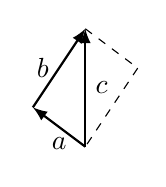
\begin{tikzpicture}
\pgfmathsetmacro{\a}{2};
\pgfmathsetmacro{\b}{1};
\pgfmathsetmacro{\c}{1.5};
\pgfmathsetmacro{\angA}{atan(\a/\c)};
\pgfmathsetmacro{\angB}{atan(\b/\c)};
\pgfmathsetmacro{\w}{0.3};
\pgfmathsetmacro{\h}{0.4};
\pgfmathsetmacro{\aa}{\c*sin(\angA)};
\pgfmathsetmacro{\bb}{\c*sin(\angB)};
%
\draw[thick,-latex](0,0)--++(90+\angA:\bb)node[pos=0.5,below]{$\bM{a}$};
\draw[thick,-latex](0,0)++(90+\angA:\bb)--++(90-\angB:\aa)node[pos=0.5,left]{$\bM{b}$}coordinate(kT);
\draw[thick,-latex] (0,0)--(kT)node[pos=0.5,right]{$\bM{c}$};
%
\draw[dashed](kT)--++(90+\angA:-\bb);
\draw[dashed](kT)++(90+\angA:-\bb)--++(90-\angB:-\aa);
\end{tikzpicture}
\caption*{(ب) سمتیوں کا مجموعہ بذریعہ متوازی الاضلاع}
\end{subfigure}%
\caption{تجربہ سے قوتوں کا مجموعہ حاصل کرتے ہوئے سمتیات کے مجموعے کا حصول حاصل ہوتا ہے۔}
\label{شکل_الجبرا_متوازی_الاضلاع_مجموعہ}
\end{figure}


\ابتدا{تعریف}\quad سمتیات کا مجموعہ\\
دو سمتیات \عددی{\bM{a}} اور \عددی{\bM{b}} کو لیتے ہوئے \عددی{\bM{a}} کے سر کے ساتھ \عددی{\bM{b}} کی دم ملائیں۔اب \عددی{\bM{a}} اور \عددی{\bM{b}} کی مجموعے کی تعریف  وہ سمتیہ \عددی{\bM{c}} ہے جو \عددی{\bM{a}} کی دم سے  \عددی{\bM{b}} کے سر تک کھینچی جائے گی (شکل \حوالہ{شکل_الجبرا_سمتیات_مجموعہ}-الف)۔اس عمل کو درج ذیل لکھا جاتا ہے۔
\begin{align}
\bM{c}=\bM{a}+\bM{b}
\end{align} 
\انتہا{تعریف}
%========================
\begin{figure}
\centering
\begin{subfigure}{0.5\textwidth}
\centering
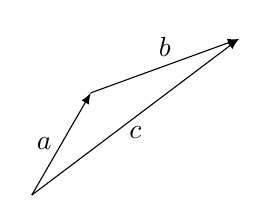
\begin{tikzpicture}
\draw[-latex](0,0)--++(60:1.5)node[pos=0.5,left]{$\bM{a}$};
\draw[-latex](0,0)++(60:1.5)--++(20:2)node[pos=0.5,above]{$\bM{b}$};
\draw[latex-](0,0)++(60:1.5)++(20:2)--(0,0)node[pos=0.5,below]{$\bM{c}$};
\end{tikzpicture}
\caption*{(الف) سر کے ساتھ دم ملا کر سمتیات کا مجموعہ حاصل کیا جاتا ہے۔}
\end{subfigure}%
\begin{subfigure}{0.5\textwidth}
\centering
\begin{tikzpicture}
\draw(0,0)--(4,0)node[below]{$x$};
\draw(0,0)--(0,2.75)node[left]{$y$};
%
\draw[-latex](0.5,0.25)coordinate(ka)--++(60:1.5)node[pos=0.5,left]{$\bM{a}$}coordinate(kb);
\draw[-latex](0.5,0.25)++(60:1.5)--++(20:2)node[pos=0.3,above]{$\bM{b}$}coordinate(kc);
\draw[latex-](0.5,0.25)++(60:1.5)++(20:2)--(0.5,0.25)node[pos=0.3,below]{$\bM{c}$};
%
\draw[dashed] (ka)--($(0,0)!(ka)!(4,0)$)coordinate(kxa)++(0,-0.6)coordinate(kkxa);
\draw[dashed] (ka)--($(0,0)!(ka)!(0,2)$)coordinate(kya)++(-0.6,0)coordinate(kkya);
\draw[dashed] (kb)--($(0,0)!(kb)!(4,0)$)coordinate(kxb);
\draw[dashed] (kb)--($(0,0)!(kb)!(0,2)$)coordinate(kyb);
\draw[dashed] (kc)--($(0,0)!(kc)!(4,0)$)coordinate(kxc)++(0,-0.6)coordinate(kkxc);
\draw[dashed] (kc)--($(0,0)!(kc)!(0,2)$)coordinate(kyc)++(-0.6,0)coordinate(kkyc);
%
\draw[thick] (kxa)--(kxb)node[pos=0.5,below]{$a_1$};
\draw[very thick] (kxb)--(kxc)node[pos=0.5,below]{$b_1$};
\draw[very thick] (kkxa)--(kkxc)node[pos=0.5,below]{$c_1$};
%
\draw[thick] (kya)--(kyb)node[pos=0.5,left]{$a_2$};
\draw[very thick] (kyb)--(kyc)node[pos=0.5,left]{$b_2$};
\draw[very thick] (kkya)--(kkyc)node[pos=0.5,left]{$c_2$};
\end{tikzpicture}
\caption*{(ب) سمتیات کے مطابقتی اجزاء کو جمع کرتے ہوئے حاصل جمع سمتیہ کے اجزاء حاصل ہوتے ہیں۔}
\end{subfigure}%
\caption{مجموعہ سمتیات۔}
\label{شکل_الجبرا_سمتیات_مجموعہ}
\end{figure}
سمتیات کی مجموعے کی تعریف سے ظاہر ہے کہ اگر کسی معین کارتیسی نظام محدد میں \عددی{\bM{a}} کے اجزاء \عددی{a_1}، \عددی{a_2} اور \عددی{a_3} جبکہ \عددی{\bM{b}} کے اجزاء \عددی{b_1}، \عددی{b_2} اور \عددی{b_3} ہوں تب حاصل جمع سمتیہ \عددی{\bM{c}} کے اجزاء \عددی{c_1}، \عددی{c_2} اور \عددی{c_3} درج ذیل ہوں گے۔
\begin{align}\label{مساوات_الجبرا_مجموعہ_سمتیات_الف}
c_1=a_1+b_1,\quad c_2=a_2+b_2,\quad c_3=a_3+b_3
\end{align}
شکل \حوالہ{شکل_الجبرا_سمتیات_مجموعہ}-ب میں اس عمل کو سطح پر دکھایا گیا ہے، اور فضا میں بھی بالکل ایسا ہی ہو گا۔

مجموعے کی تعریف یا مساوات \حوالہ{مساوات_الجبرا_مجموعہ_سمتیات_الف} سے مجموعہ سمتیات کی درج ذیل خصوصیات ملتی ہیں جہاں \عددی{-\bM{a}} سے مراد ایسا سمتیہ ہے جس کی لمبائی \عددی{\abs{\bM{a}}} اور سمت \عددی{\bM{a}} کے الٹ ہو۔
\begin{gather}
\begin{aligned}
\text{(الف)}\quad \quad \bM{a}+\bM{b}&=\bM{b}+\bM{a}\quad \text{\RL{قانون تبادل}}\\
\text{(ب)}\quad (\bM{u}+\bM{v})+\bM{w}&=\bM{u}+(\bM{v}+\bM{w})\quad \text{\RL{قانون تلازم}}\\
\text{(پ)}\quad \quad \bM{a}+\bM{0}&=\bM{0}+\bM{a}\\
\text{(ت)}\quad \quad \bM{a}+(-\bM{a})&=\bM{0}
\end{aligned}
\end{gather}

